\section{Voltage Error Amplifier}

\begin{figure}[H]
\centering
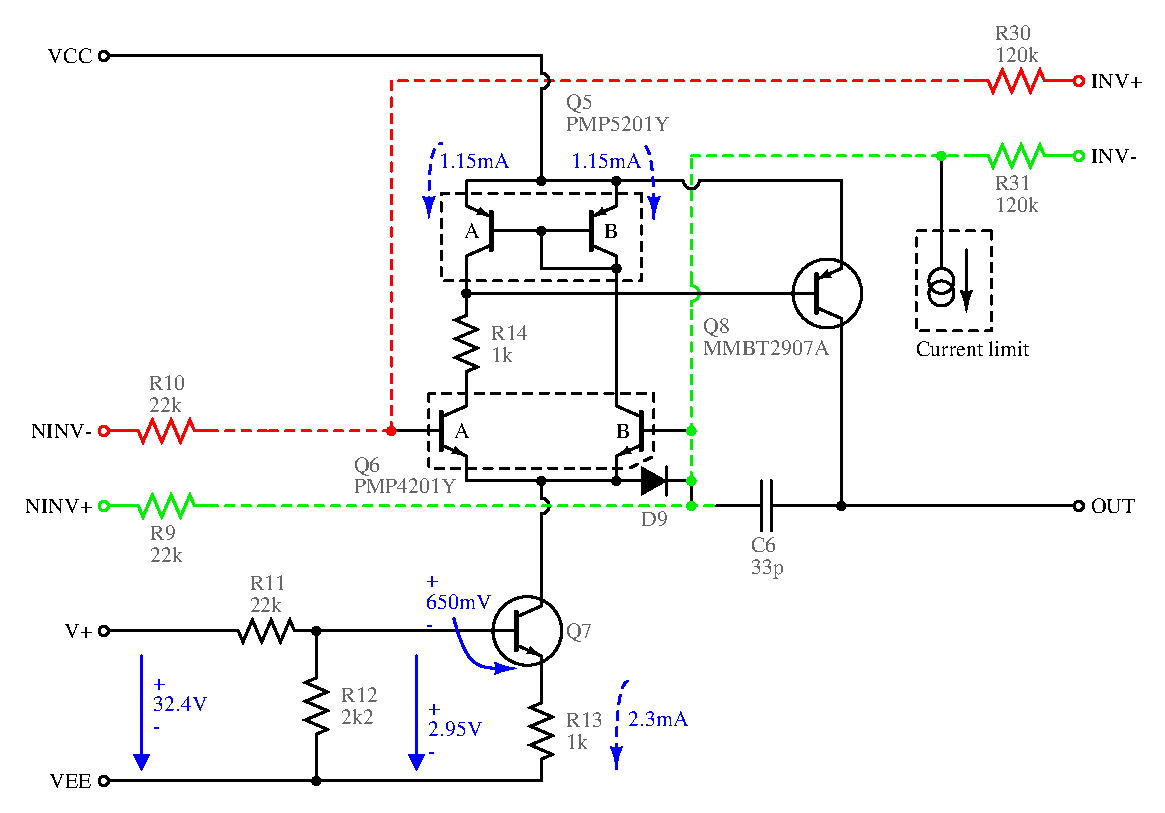
\includegraphics[width=5.5in]{sch/verror}
\caption{Voltage error amplifier sub-schematic}
\label{fig:verror}
\end{figure}

\begin{multicols}{2}

An error amplifier is a circuit which compares a reference level to the
actual output, adjusting the output driver according to the amount of error
present. This is done simply by subtracting the output level from the
reference level, amplifying the difference by a large amount, and using
this directly to control the output.

The error amplifier shown above is based on a transistor arrangement
called a ``long-tailed
pair'' or ``differential pair'' (Fig. \ref{fig:ltp}). This is the heart of
most differential circuits, including the operational amplifier.


\begin{figure}[H]
\centering
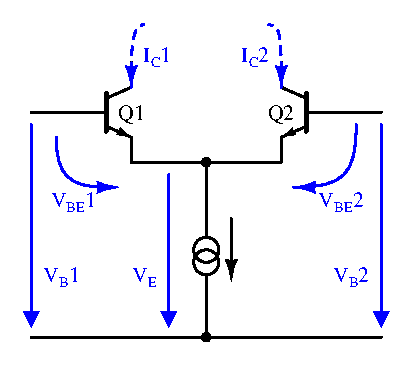
\includegraphics[width=2in]{sch/ltp}
\caption{Long-tailed pair}
\label{fig:ltp}
\end{figure}

\subsubsection{Long-Tailed Pair}
I will spare you the mathematics of fully analyzing the long-tailed pair,
because it is very easy to explain without numbers. Imagine the saturated
case. This is where the two input voltages, $V_{BE}1$ and $V_{BE}2$, are
vastly different, so the output is as large as it possibly can be. Suppose
$V_{BE}2$ is significantly greater than $V_{BE}1$. The voltage at the
emitters, $V_E$, must be one B-E drop less than $V_{BE}2$. This is because if
it were any lower, \texttt{Q2}'s B-E diode would be forward biased, and would
begin to conduct. So \texttt{Q2} will be conducting, with $I_C2 > 0$, and
\texttt{Q1} will not conduct, with $I_C1 = 0$, because its B-E diode will not
be forward biased. Therefore, the current draw into the transistors is
determined by which of the two voltages is larger. This is a comparator.

If $V_B1$ and $V_B2$ are very close, both transistors will conduct, with
the one having a larger $V_{BE}$ conducting more. $V_E$ will be determined
by both base voltages, and since $V_{BE}$ is just $V_B - V_E$, the current
into each transistor will be determined by the \emph{relative} voltage
between the bases. This is a proper differential amplifier.

\subsubsection{Sources of Error}
The voltage error amplifier must be a \emph{precision} amplifier. 
A matched pair, \texttt{Q6}, is used, to make sure the gains and
threshold voltages on each side are the same. Still, there is more variation
that must be corrected. First, if the two transistors draw significantly
different currents, their gains and thresholds change. \texttt{Q5} is another
matched pair, acting as a current mirror. \texttt{Q5B} is diode-connected,
so that current may be drawn through it, and \texttt{Q5A} is
transistor-connected to the same $V_{BE}$, so that it will pass the same
current. This stabilizes the current difference between the two, and
\texttt{Q7}, a simple current source, stabilizes the total current.

An error amplifier must have extremely high gain in order to be precise.
This is because its operation \emph{depends} on a small error being present.
Higher gain means it will be sensitive to a smaller error.
\texttt{Q8} is connected as a simple common-emitter amplifier
to provide voltage gain to the output.

\subsubsection{Feedback Mechanism}
Feedback paths are colored in Figure \ref{fig:verror}. 
{\small \it Note: If you are reading a
greyscale copy, the paths have been marked with dashed lines; the red path
lies on top and runs through \texttt{R10}, and the green path lies underneath
and runs through \texttt{R9}.}
The red path is
noninverting: if the voltage on that path is increased, the voltage on
\texttt{Q8}'s collector (the output) will also increase. The green path
is inverting. As an example of the corrective action of the circuit: Imagine
that there
is voltage loss in the positive output lead's resistance.
The noninverting path will fall (as the positive output lead is connected
to ``INV+''),
and ``OUT'', which drives the \emph{negative}
output lead, will fall in turn. The overall output voltage will increase,
compensating for the drop in the positive lead.

\texttt{C6} exists to slow down the error amplifier. If the output drops
too quickly, \texttt{C6} will begin to conduct, pulling down the inverting
path, and therefore pulling the output back up. This is necessary for
stability. Without it, the error amplifier can operate faster than the
lag of the feedback system, causing it to ``see'' a delayed reading and
leading to oscillation.

\subsubsection{External Cutoffs}
Both the current limiter and the thermal cutoff shut down the output by
pulling the inverting path down (thus pulling the negative output up). If the
path is pulled below the emitter voltage of \texttt{Q6}, \texttt{Q6B}'s B-E
junction will be reverse biased, which can cause damage. \texttt{D9} limits
this reverse bias to -0.7\;V. Unfortunately, this provides a path for
unlimited current (through \texttt{Q8} E-B, then through \texttt{Q6A} C-E,
then through \texttt{D9}), so \texttt{R14} is installed to limit the current.

\end{multicols}
